The first method we try is something really simple. We purely look at the Sharpe Ratio, we simply look for strategies that satisfied a certain requirement in the past and eventually select them based on the current Sharpe ratio over a certain window. More in detail, every week we scan the whole universe of strategies and we apply the aforementioned Sharpe-filter, pre-selecting only the ones that had a "good enough" performance over a certain window in the past. This period can be not in the near past. That means this is a strategy that somehow has proven to be an alpha generator in the past at least. After this pre-selection we put in production only the strategies that currently have a Sharpe-ratio over a certain window greater than a fixed threshold. For this method to work properly we need to fit four parameters (two thresholds and two windows for the Sharpe Ratio). Even though we might let the optimizer work on an infinite space, we set some boundaries to our search. For example, we will require the Sharpe filter to work over a longer period (at least 6 months). While the shorter Sharpe, will be based on a shorter window that will not exceed one trading year.\\
We run the in-sample grid search and nicely find a smooth surface. This is good news because it confirms that we are not chasing the noise but generating a real signal. 

\begin{center}
	\centering
	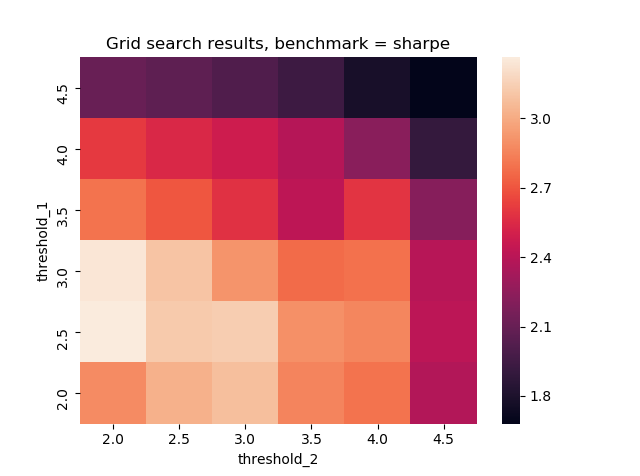
\includegraphics[width=0.6\textwidth]{GridSearches/Sharpe_Basic/Figure_1.png}
	\captionof{figure}{Grisearch results for the two thresholds}
	\label{Sharpe_Simple_1}
\end{center}

\begin{center}
	\centering
	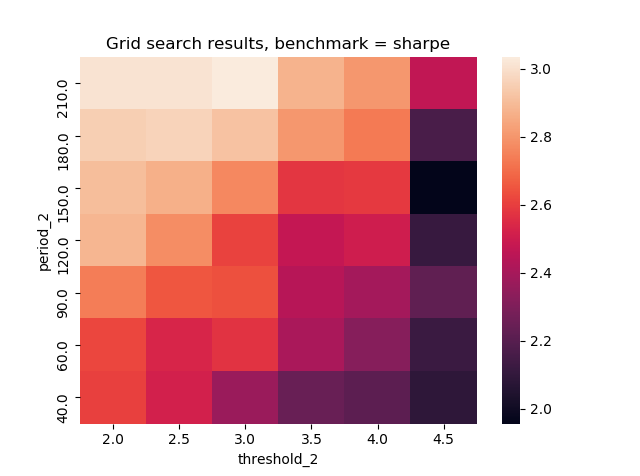
\includegraphics[width=0.6\textwidth]{GridSearches/Sharpe_Basic/Figure_2.png}
	\captionof{figure}{GridSearch for the threshold and period relative to the short Sharpe-Ratio}
	\label{Sharpe_Ranking_2}
\end{center}

\begin{center}
	\centering
	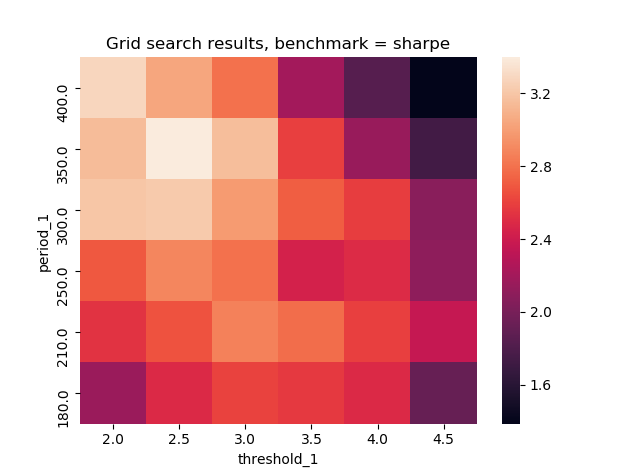
\includegraphics[width=0.6\textwidth]{GridSearches/Sharpe_Basic/Figure_5.png}
	\captionof{figure}{GridSearch for the threshold and period relative to the long Sharpe-Ratio}
	\label{Sharpe_Ranking_2}
\end{center}

The way these graphs should be interpreted is that for each point in the grid we see a value that is the average on all the possible values of the non displayed parameters. Otherwise we would have to draw somehow an n-dimensional cube, but for simplicity and visibility we prefer to plot everything on a 2D surface.\\

The results are definitely interesting. Since we don't care about finding exactly the perfect optimal combination of parameters we stick with what we believe makes sense in the optimal area that means longer Sharpe ratio over a period of 350 days and shorter Sharpe computed over a period of 210 days.